\section{Introduction}
\label{sec-introduction}

\begin{figure}
	\centering
	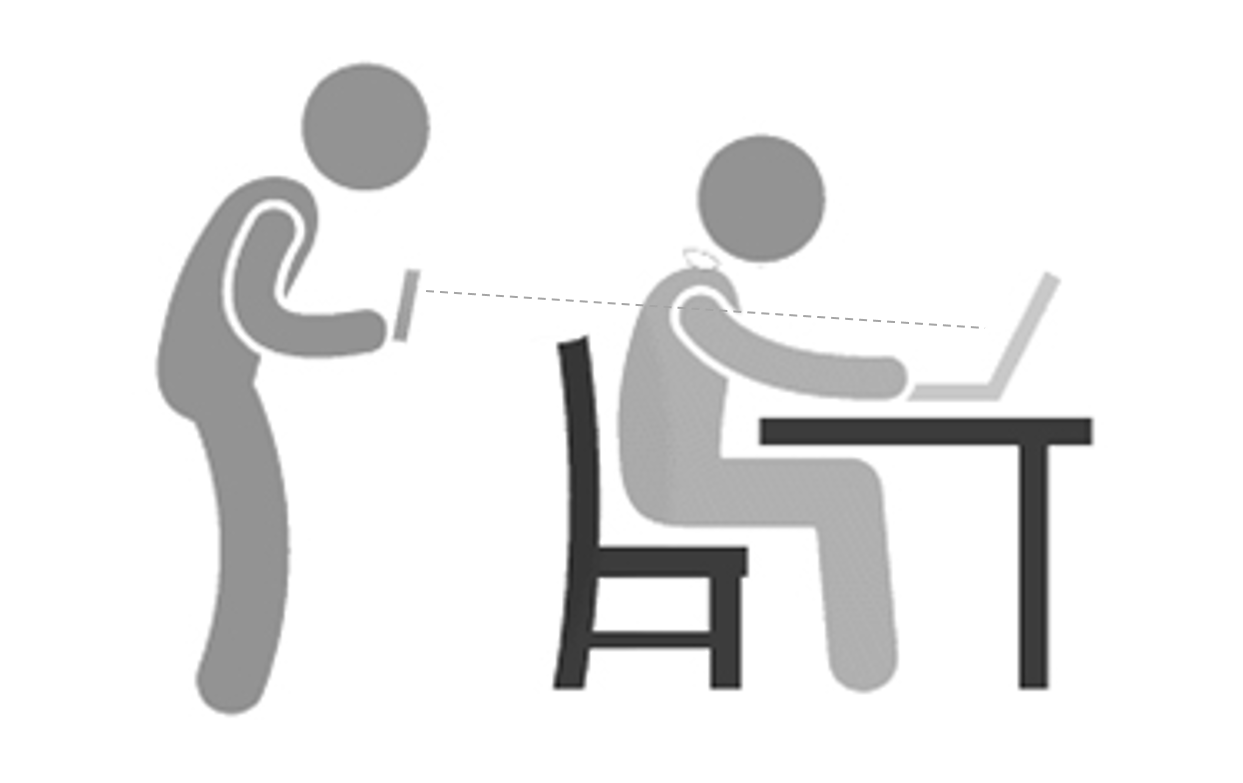
\includegraphics[width=0.48\textwidth]{pic/intro.png}
    \caption{Overview of the proposed shoulder surfing threat model.}
	\label{fig-zeros}
\end{figure}
% introduce LPL asynchronous duty cycle media access
As already we are aware, smartphones have become a necessity in our lives, as we are checking our mobile phones constantly throughout the day. As a result, some privacy concerns have arisen about nearby parties peeking at our screen, namely ``shoulder surfing". 
Assuming that the attacker is not malicious and merely takes several peeks out of curiosity, most works in this area are built on a threat model of an attacker observing with naked eyes. And studies show that a great portion of these attacks are casual and opportunistic without technical equipment~\cite{eiband2017understanding}, say a mere stranger can hardly do any harm reading a fragment of the correspondence or acquiring the password without knowing the account for critical apps like Alipay, which seldom appears on screen in common usages. 
% It is however the rare but malicious attacker, with certain familiarity and knowledge of the victim, that can do the most harm. The attacker can even be our closest friends or family members, as there are various cases in China where a child obtains Alipay password of their parents and is unaware that electronic payments consists of 'real' money, resulting in spending them lavishly in their games. Besides, specially designed equipment are not a necessity for the shoulder surfing attack. 

The privacy threat however has been exacerbated with smartphones improved significantly these years. Given the commercial smartphone, the attacker can not only reduce suspicion by acquiring sensitive information from a long distance, but also record the information for propagating, rendering greater damage to the victim. For example, in a Senate hearing, the Justice Secretary of Philippines, Vitaliano Aguirre II, suffered a leakage of his text messages, as someone had taken a snapshot of his smartphone \cite{Polotiko2017leakage}.Equipped with multiple cameras, the newest generation of smartphones can perform 100$\times$ zooming compared to the standard 5$\times$ of single camera phones. Hardware improvements in memory also allows the burst mode at tremendous frame rates and even high-speed photography, delivering videos with thousands of frames per second. And more images means more recorded information of the victim. To gain vital data stealthily from even further away, the processing technique of multi-frame super resolution (SR) algorithms can be employed by the attacker, delivering a more threatening shoulder surfing model.

% In this present era where the leakage of a password and the disclosure of correspondence of public figures can cause great damage to the victim, we believe that it's imminent to recall attention on this new privacy threat and propose the corresponding standard of screen protection based on modern circumstances.

To mitigate this threat, massive efforts have been made, from physical privacy films to alternative password entry interfaces \cite{wiedenbeck2006design,papadopoulos2017illusionpin} and input methods \cite{kumar2007reducing}. All of these methods however require additional cost and/or effort \cite{Chun2019Keep} and are not widely deployed yet on the critical privacy stages (e.g., password entry) of most everyday apps. And none of existing work can deal with the presence of smartphone cameras and SR algorithms in shoulder surfing scenarios. Given that the leakage of a password and the disclosure of correspondence of public figures can cause great damage to the victim, we believe that it's imminent to recall attention on this new privacy threat and propose the corresponding standard of screen protection based on modern circumstances.

\cl{The challenge part can be revised to make it more precise. And it can be described with the new figure.}
\vspace{1mm}
\noindent
\textbf{challenges.} Creating a high-resolution shoulder surfing attack model running on commercial smartphones in real time, however, is not trivial. And we achieve \textsf{SRPeek} by overcoming three key challenges.
\begin{figure}
	\centering
	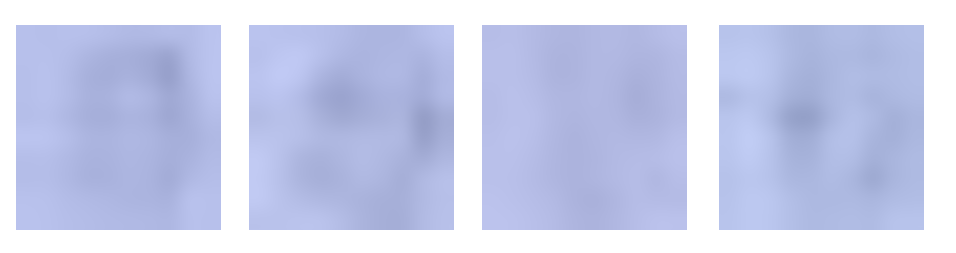
\includegraphics[width=0.48\textwidth]{pic/zeros.png}
    \caption{Photos of number ‘0’ on a screen at a distance of 1.5m, taken in quick succession from a still smartphone camera. All exhibit different blurriness and no consistency between neighboring frames.\cl{Figure should be replaced.}}
	\label{fig-zeros}
\end{figure}
\begin{itemize}[leftmargin=*]
  \item \textbf{Blurriness of input images.} \cl{need revising.} The most prominent one is the blurriness, as our photos are taken at extreme range, taken secretly and hurriedly without much room for focusing, while straining the magnification of the smartphone lenses. Unlike most SR applications and datasets working with ‘normally’ captured photos, the images we face exhibit lower concentrations of information and more artifacts, and needs more ‘reconstruction’ than ‘interpolation’. \cl{However, such blurry input means less information, and a greater possibility of reconstructing the wrong character. In deep learning based methods, a deep network often leads to gradual divergence from the truth as the data is propagated deeper through the network pipeline, resulting in 'fake' high-res images, especially when the subjects are the discrete strokes of characters, instead of details and texture of everyday objects. As a matter of fact, most works on multi-frame SR function on video clips \cite{lucas2019generative} or multiple snapshots \cite{wronski2019handheld}, however, our application is subtly different from the two. Our dilemma is as follows: on one hand, each one of the photos we are to process is blurred with a randomly different PSF kernel, which, because of the extreme blurriness, cannot be approximated as a constant, isotropic gaussian kernel, and thus lacking consistency between neighboring frames, meaning that they cannot be processed as a video clip(see Fig.~\ref{fig-zeros} ); on the other hand, because of the low concentration of information, the blurred photos are similar to pieces of a jigsaw puzzle, each containing only fractions of information, and the only chance of recovering the ground truth is by comparing each photo against others. If processed by common procedures enhancing the resolution of a series of snapshots—processing each one separately and merging them afterwards, few useful information can be extracted from each one of the images, and merging them will not produce satisfactory results.}	
  \item \textbf{Processing with multiple frames.} While exploring this privacy threat, we need a multi-frame SR algorithm on a smartphone to monitor the target phone in real time. However, we discover that there is no existing SR algorithm suitable for this scenario. On one hand, images captured by hand are blurred while most methods rely on a handful of clearer images (e.g., scenery, scanned images) \cite{nasrollahi2020deep,lyn2020image}. Specifically, we have to extract the information from large quantities of extremely blurred photos, as smartphones can capture 10 snapshots per second in burst mode, and these photos are taken from extreme distances. On the other hand, the difference between videos and multiple snapshots rules out the video super resolution algorithms, which cannot be adapted to larger numbers of input images. The reason has two folds. First, either increased input leads to increases in model complexity, making it unsuitable for mobile deployment. \cl{Second, most models rely heavily on the information extracted from each single image, however, the images in our application are so blurry and distorted that we cannot tell if, for example, it is one stroke or two parrallel strokes that is shown in these two darker pixels on this photo---unless we consult pixels at the same location in other input photos. The nature of our task requires this kind of consultation of pixels with same coordinates on different images throughout our construction process, and this mechanism needs to be designed into the network architecture.}
  \item \textbf{Model complexity and variable input.} \cl{To achieve real-time monitoring, we need to perform our calculations locally on the smartphone, instead of sending the data to a server and process them remotely, because 1) the latter would require stable Internet access, and 2) sending multiple images across the Internet will consume time and bandwith. However, to get ideal results we need 10 to 20 images which will consume 1 to 2 seconds to capture, and this time period is the minimum interval between each output frame, with the processing phase working in parrallel. This way the time allowed for calculation is 1 to 2 seconds, with limited calculation power and RAM. In cases where the display on the target screen changes more frequently, less images will be avaliable for each scene, and the attacker requires more frequent feedback which means less time for each processing task. These not only require a smaller and simpler network model, but also a model that can function with variable input, efficiently utilizing the data from either 3 or 20 images and provide results to the best of its efforts.} 
  \item \textbf{Complexities of characters.} As the information of interest in shoulder surfing scenarios is mostly in the form of text (e.g., passwords or e-mails), we will focus on reconstructing text, specifically, Chinese characters, English letters, and numbers, in our system.\cl{declare this beforehand?} The task of reconstructing text, instead of scenary or objects, poses unique challenges. Composed of multiple strokes, these characters are distributed discretely in image space, not known to other entities, e.g. faces and natural objects. In some cases, messing up a stroke will not impact its readability, and in other cases shortening or lengthening a stroke even slightly will lead to a different character, leading to misunderstandings. And unlike most SR applications working on similarity (between their output and the ‘ground truth’), our goal is readability, and the network architecture and training process must be engineered accordingly.\cl{ Another challenge is imbalanced data. Among Chinese characters certain strokes and stroke groups are always more commonplace than others, and this imbalanceness often results in lower prediction accuracy over the less common,  unconventionality shaped characters. On the other hand, however, the focus on characters can also aid us. As our network is only expected to reconstructe these characters, the network can learn to detect features from the input and reconstruct strokes and segments from them, extracting more information from the blurry images.}
\end{itemize}
  


\cl{The following part can correspond to challenges above. Remember to be precise and illustrative.}
In this paper, we present \textsf{SRPeek}, an end-to-end system of shoulder surfing for commercial smartphones. Deployed on a smartphone, this system will take snapshots of the target screen in burst mode of the attacker's screen, which are aligned, cropped, and then processed by our multi-frame SR neural network to generate a high-res image of the victim's screen. The core of this system, the nerual network, is specifically designed and trained for this task, aimed to counter the four challenges mentioned above. The outline of this network is as follows:
\begin{itemize}[leftmargin=*]
  \item \textbf{Layered architecture and frequent introduction of input.} To counter the blurriness of the images, and the tendency of reconstructing fake characters, our network is constructed with several identical SR layers, connected sequentially, and the images are refined step by step throughout the layers. The input and output of each layer is also correspondent to each avaliable image\cl{???}, as all input images are processed simultaneously and separately(with the information from other images for reference) throughout the network, all the way to the end of the model where we merge all the data into one output image. Another importent feature of our architecture is that the initial input images are introduced into the dataflow at each layer, from beginning to end, resulting in the uneven depth of our model, acting as an anchor for the reconstruction process so that the output will be faithful to truth from beginning to end, while preserving the deep mainstream of the model to be able to process such blurry images.
  \item \textbf{Merging layers to adapt multiple frames.} The SR layer consists of several convolutional layers and a specially designed merging layer, which is the sole revenue of communication across images. As mentioned above, these images are processed individually thouroughout the network, and they are inputted from the last layer independently, convolutioned independently, and passed to the next layer independently. This apparently cannot fully utilize the information across the multiple frames, so that we design a merging process inside each SR layer, which merges featuremaps from all the images into one, and this data is distributed to each image in this layer and stacked with their featuremaps for the next convolution. In this way, during the refinement process of each of the images in every SR layer, the model has access to data of consensuses among other contemporary images, which can inspire the network to extract more prominent and collective features, and induce the convergence of all input images for increased seamlessness at the successing merging layer. In most deep learning architectures, the features extracted in each layer is more complex than the previous ones, the former's discoveries built on what the latter has achieved, and our model is not an exception; However, the merging layers we designed can support this increase. At each layer the image is exposed to the consensuses of features from other images at the same level of complexity, acting as a verification for the hypothetical features extracted from the current image, so that in the training process more audacious features can be learned and proposed without fear of punishment from the final loss, increasing the quality of featuremaps throughout the network.
  \item \textbf{Model Complexity and adaption for variable input.} All the convolutional layers throughout the network are thus designed: They are performed individually for each image(or the featuremaps of them from the previous layer), and these convolutions in the same layer share a same set of parameters in training and production, thus reducing parameter count and avoiding convolutions for large numbers of channels, saving calculation power. This also leads to the benefit that the output featuremaps of all the images are the evaluations over the same set of features\cl{???}, so that the merging process can also be accomplished easily without the need of trainable parameters. In our design, the merging layers consists of simple pixelwize processes resembling average, min and max processors, to filter out either the collective or the most prominent features among the featuremaps. This process functions with any number of input images. As the convolutional processes are also performed individually for each layer, the same set of parameters of the network model can function normally with any number of input images, while the calculation complexity also increases linearly with the amount of input. On one hand, this gives our model the ability to adapt to the uncertainty of the number of avaliable images, providing relatively satisfactory results regardless whether the attacker has ample time photographing the target phone before it changes its display; on the other hand, the relative independence and the isotropy of the merging layers avoids the reliance on sequential order and consistency between neighboring frames(which is common among most multi-frame SR networks), solving the inconsistency problem mentioned in Fig.~\ref{fig-zeros}.
  \item \textbf{Compatibility with complex characters.} The discrete distribution of characters leads to the inclination of diviation and producing 'fake' results. The frequent introduction of input images is designed to mitigate this challenge. Also, our model is trained on these characters---the images we collected for the training dataset are all cropped so that only the characters remain, so that during the training processes the model can learn correlations between certain features and strokes, and the regular patterns of the characters, narrowing the possibilities offered by the blurry images. We also introduce adaptive boosting\cite{adaboost} in our training process, increasing the loss weight of the wrongly reconstructed characters, determined by loss in earlier stages and OCR in later stages, to accommodate the imbalanceness of data. The loss functions in training is also redesigned. The mean square error(MSE) is not suitable in this application, as a misplaced stroke, although highly obstructing readability, may only invoke a slight decrease in MSE because it only influenced a few pixels. Our solution is putting a weight on each pixel before applying weighted MSE. Assuming the characters are black on white, this weight increases at darker pixels and propagates to neighbouring dark pixels so that long strokes and intersections of strokes are given higher weights. This process serves as a supplement to MSE to focus more on readability and is beneficial for OCR and human reading tests. 
\end{itemize}



\cl{Evaluations can be summarized here (performance and comparison with existing works).}

\vspace{1mm}
\noindent
\textbf{Summary of Evaluation Results.}


\vspace{1mm}
\noindent
\textbf{Contributions.} This paper makes the following contributions:
\begin{itemize}[leftmargin=*]
  \item	We propose \textsf{SRPeek}, a multi-frame SR neural network architecture aiming at reconstructing extremely blurred and defocused images. This model is not only functional in our scenario, as a shoulder-surfing threat model, but also can be used in text-recognition applications prior to recognition algorithms to increase accuracy.
  \item	We design a threat model of shoulder-surfing, with the attacker armed with multi-frame SR algorithms and taking multiple photos (in burst mode) of the victim’s screen with a smartphone camera. To the best of our knowledge, we are the first to consider the presence of smartphone cameras and SR algorithms in shoulder surfing scenarios.
  \item	We demonstrate the effect of this shoulder-surfing attack and prove that it poses a threat to screen privacy.
\end{itemize}

% describe the organization of the paper
The rest of the paper is organized as follows. Section 2 describes the threat model of our  carefully studies the performance of state-of-the-art concurrent flooding. The detailed design of COFlood protocol is shown in Section~\ref{sec-design}. We show the implementation details and evaluation results in Section~\ref{sec-implementation-and-evaluation}. The related work is introduced in Section~\ref{sec-related-work}. Finally, we conclude our work in Section~\ref{sec-conclusion}.
